\documentclass[13pt,a4paper]{article}
\usepackage[utf8]{inputenc}
\usepackage{setspace}
\onehalfspacing
\usepackage{enumerate}
\usepackage{hyperref}
\usepackage{float}
\floatstyle{boxed} 
\restylefloat{figure}
\usepackage{amsmath}
\usepackage{mathrsfs}
\usepackage{color}
\usepackage{graphicx}
\usepackage{adjustbox}
\usepackage[left=1cm,right=1cm,top=2cm,bottom=2cm]{geometry}
\usepackage{fancyhdr}
\pagestyle{fancy}
\fancyfoot{}
\fancyhead{}
\fancyfoot[R]{\thepage\ }
 \renewcommand{\headrulewidth}{2pt}
 \renewcommand{\footrulewidth}{2pt}
\fancyhead[L]{Class: EE 228}
\fancyhead[R]{Hadi Asemi}
\fancyhead[C]{Signal and Systemss}
\newlength\FHoffset
\setlength\FHoffset{1cm}
% \addtolength\headwidth{2\FHoffset}
% \fancyheadoffset{\FHoffset}
% \fancyfootoffset{\FHoffset}

\usepackage{multicol}
\setlength{\columnseprule}{0.4pt}
\def\columnseprulecolor{\color{blue}}
\usepackage{float}
\title{Formula Sheet EE228}
\author{hadiasemi }
\date{October 2019}

\begin{document}
\begin{titlepage}
	\begin{center}
		\line(1,0){300}\\
		[0.25in]
		\huge{\bfseries EE 228}\\
		[2mm]
		\line(1,0){300}\\
		[1.5cm]
		\textsc{\LARGE Signals and Systems}\\
		[1.5cm]
% 		\includegraphics[width=70mm]{Image/7.jpg}
		\textsc{\Large Fred DePiero}\\
		[14cm]
		
	\end{center}
	\begin{flushright}
		\textsc{\large Hadi Asemi\\
		 %G01049243\\
	    	\today\\}
	\end{flushright}
\end{titlepage}
	
\cleardoublepage
\tableofcontents
\thispagestyle{empty}
\cleardoublepage
\setcounter{page}{1}

% \begin{multicols}{2}


% \begin{gather*}
% \textbf{Usefull integrals:}\\
% \int^T_0 \sin{n\omega t} dt=0\\
% \int^T_0 \cos{n\omega t} dt=0\\
% \int^T_0 \sin{n\omega t}*\cos{n\omega t} dt=0\\
% \int^T_0 \cos{n\omega t}*\cos{m\omega t} dt=0\\
% \int^T_0 \cos^2{n\omega t} dt=\frac{T}{2}\\
% \int^T_0 \sin^2{n\omega t} dt=\frac{T}{2}\\
% \end{gather*}
% %  \columnbreak
 
%  \begin{align*}
%  addititve &\rightarrow \large{ O\{x_1(t)+x_2(t)\}=O\{x_1(t)\}+O\{x_2(t)\}}\\
%  homogeneous &\rightarrow O\{Kx(t)\}=KO\{x(t)\}\\
%  \end{align*}

% \end{multicols}
%  \begin{multicols}{2}
\setcounter{section}{0}
\setcounter{subsection}{1}

\section{Operations on Signals:}
\begin{align}
    y(t)&=Cx(t)\rightarrow{\text{increase the amplitude}}\\
     y(t)&=x(t-\alpha)\rightarrow{\text{shift the signal x(t)}}\\
     y(t)&=x(t/2)\rightarrow{\text{expansion of x(t)}}\\
     y(t)&=x(2t)\rightarrow{\text{compression of x(t)}}\\         y(t)&=x(-t)\rightarrow{\text{\small{create mirror image signal about the vertical Axis}}}\\
\end{align}
\textbf{Important:} for calculating the graph new equation we need use the $C_1t_1+D_1=t_0$.\\
$
    t_0=\frac{-D_0}{C_0}
$
\section{Symmetry (Odd and Even Functions):}
\textbf{Note:} if the a signal is identical to its folded version, with \textbf{x(t)=x(-t)}, it is called \textbf{Even Symmetric.} If a signal and its folded version different only in sign, with \textbf{x(t)=-x(-t)}, it is called \textbf{Odd Symmetric.}\\
\begin{gather*}
    odd=\int_{-\alpha}^\alpha x_0(t)dt=0\\
    even=2\int_{0}^\alpha x_0(t)dt\\
\end{gather*}
\textbf{Important:}
\begin{align*}
    x_o*y_o&\rightarrow{Even}\\
    x_e+y_o&\rightarrow{\text{No symmetry}}\\
    x_e*y_o&\rightarrow{Odd}\\
    x(t)&=x_e(t)+x_o(t)\\
    x_e(t)&=0.5[x(t)+x(-t)]\\
    x_0(t)&=0.5[x(t)-x(-t)]\\
\end{align*}

\section{Sampling (or shifting) property:}
\begin{gather*}
    \int_{-\infty}^{\infty}x(t)\delta(t-\tau)dt=x(\tau)\\
    \delta(at)=\frac{1}{|a|}\delta(t)
\end{gather*}
\textbf{Note:} Always check the boundary of the integral for $\delta(t-\tau)$ because if is not in the boundary the integral would be zero.\\
Example:
\begin{gather*}
    \int_{-3}^{-1}t^5\delta(3t+2)dt\\
    \frac{1}{3}*(\frac{-2}{3})^5\int_{-3}^{-1}\delta(t+\frac{2}{3})dt=0\rightarrow \frac{-2}{3}\ne -3<t<-1
\end{gather*}
\section{Linearity:}
Check homogeneity and superposition and if we have anything like $x^2, y^2, x*x^{'},a^{y}$.\\

\section{Causality:}
An LTI system is cuasal if and only if its \textbf{impulse response} is a causal function. $h(t)=0 for t<0$
\begin{enumerate}[I)]
    \item Does a system respond before an input accrues\\
    \item Does these system rely on future input.\\
\end{enumerate}
\begin{align*}
     y(t)&=x(t+2)\rightarrow \text{It is depend of future event, so non-causal}\\
    y(t) &=x(3t)\rightarrow \text{expansion and compression}
\end{align*}
%  \section{Introduce impulse response:}
% \begin{gather*}
% x(t)=\delta(t)    
% \end{gather*}
\section{Dynamic vs Static(instantaneous):}
\textbf{Dynamic} system contain Energy element describe by $\frac{d}{dt} or \int dt$.\\
\textbf{Static} if the output $y(t_0)$ depends only on the instantaneous value of the input $x(t_0)$ like y(t)=Ax(t)+B. It is \textbf{static} if no derivatives are present, and every term in x and y has identical arguments.\\
\begin{align*}
    y(t)\ne x(t+1)\rightarrow Dynamic
\end{align*}
Because the input value for the y and x are different.
\section{ Time-Invariant (Shift-Invariant) Systems:}
Time-scaled inputs or outputs also make a system equation time varying as with y(4t).
\begin{align*}
    O\{x(t-t_0)\}=y(t-t_0)\rightarrow \text{(shift input by $\alpha \rightarrow$ shift output by $\alpha$)}
\end{align*}
To be time invariant, coefficients of the differential equation \textbf{cannot} be function of time, such as $3ty^{'}$.

\section{Stability:}
Stable if any "bounded" input x(t). \\
$|x(t)|<m_x$ for all t $m_x<\infty$ also the output is also bounded $|y(t)|<m_y  , m_y<\infty$.\\
\begin{enumerate}[I)]
    \item The degree of the highest derivative of x(t) must not exceed that of the highest derivative of y(t).
    \item Every root of the characteristic equation must have a negative real part.
\end{enumerate}
\textbf{Example:}
\begin{gather*}
    y^{''}(t)+3y^{'}(t)+2y(t)=x(t)
\end{gather*}
Stable because the roots of characteristic equation $s^2+3s+2=0$ are s=-1,-2 and have a negative real part.
\section{Even and Odd Functions:}
\begin{align*}
    X_e(t) &=0.5[x(t)+x(-t)]\\
    X_o(t) &=0.5[x(t)-x(-t)]\\
    X(t) &=x_e(t)+x_o(t)
\end{align*}
% \begin{figure}[H]
%     \centering
%      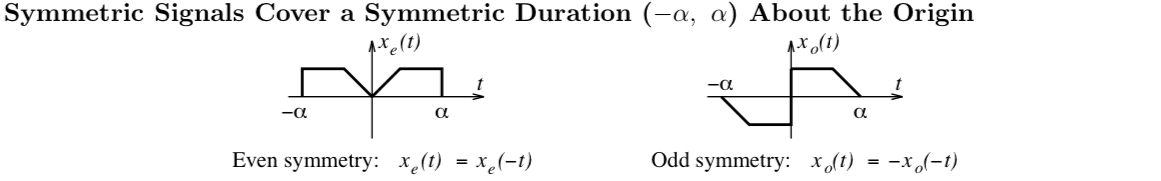
\includegraphics[width=170mm]{2.jpg}
%     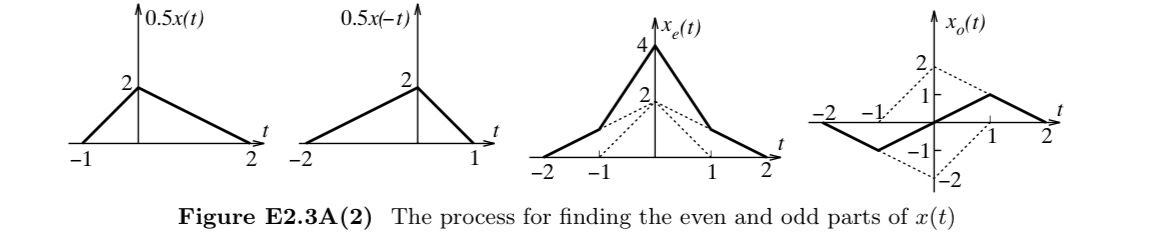
\includegraphics[width=150mm]{1.jpg}
%     % \caption{Caption}
%     % \label{fig:my_label}
% \end{figure}
\section{DC Average $\&$ RMS :}
\begin{align*}
    E &=\int_{-\infty}^{\infty}|x(t)|^2dt\\
    P_{DC_{avg}} &=\frac{1}{T}\int^{t_0+T}_{t_0}v(t)dt\\
    P_{avg} &=\frac{1}{T}\int^{t_0+T}_{t_0}v(t)^2dt\\
    P_{rms} &=\sqrt{P_{avg}} 
\end{align*}
% \section{Linear constant coefficient differential Equations(LTI):}
\section{Convolutions:}
The notation for convolutions is $x(t)\star h(t)$.
\begin{align*}
    y(t) =x(t)\star h(t) &=\int_{0}^{t}x(\lambda)h(t-\lambda)d\lambda\\
    u(t)\star u(t) &=r(t)\\
    rect(t)\star rect(t) &=tri(t)\\
    e^{-\alpha t}u(t) \star e^{-\alpha t}u(t) &=te^{-\alpha t}u(t)
\end{align*}
% \begin{figure}[H]
%     \centering
%     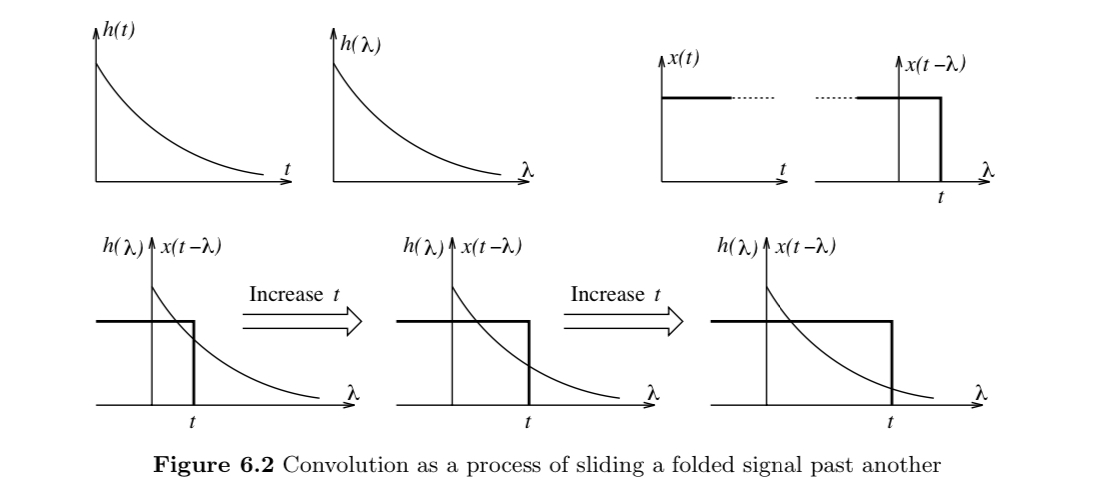
\includegraphics[width=20mm]{3.jpg}
%       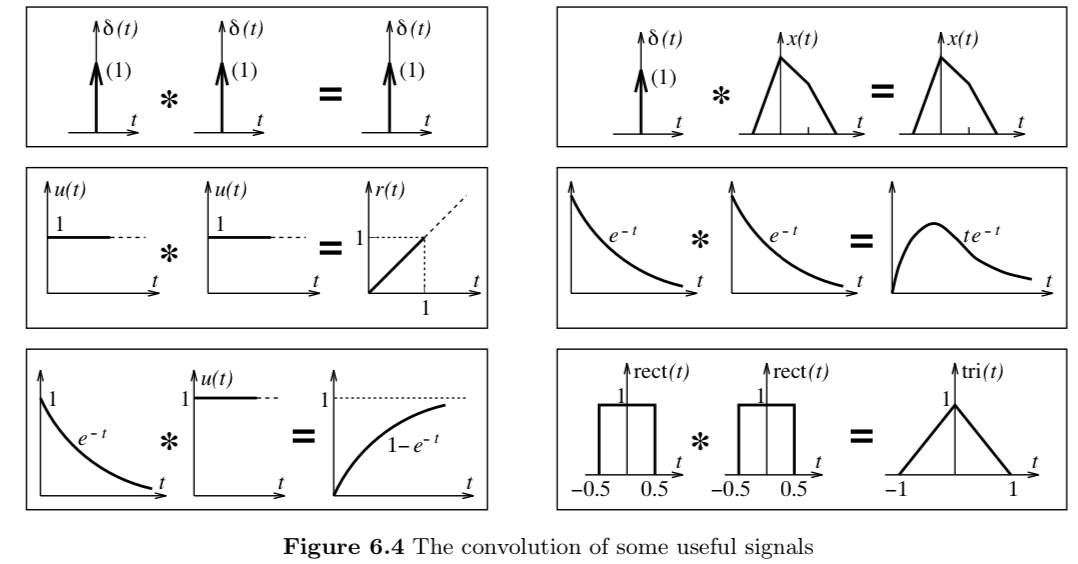
\includegraphics[width=20mm]{4.jpg}
%     % \caption{Caption}
%     % \label{fig:my_label}
% \end{figure}
The convolutions of any signal h(t) with impulse reproduce the h(t) signal.
\begin{gather*}
    \delta(t)\star h(t)=\delta(t)
\end{gather*}
\section{The Natural, Forced, and Total Response:}
Total Response = Natural Response + Forced Response\\
The roots of the characteristic equation determine only the form of the \textbf{natural} response.\\
The input terms (RHS) of the differential equation completely determine the forced response.\\
Initial conditions satisfy the total response to yield the constants in the natural response.\\
The \textbf{forced response} arises due to the interaction of the system with the input and thus depends on both the input and the system details.
% \begin{figure}[H]
%     \centering
%     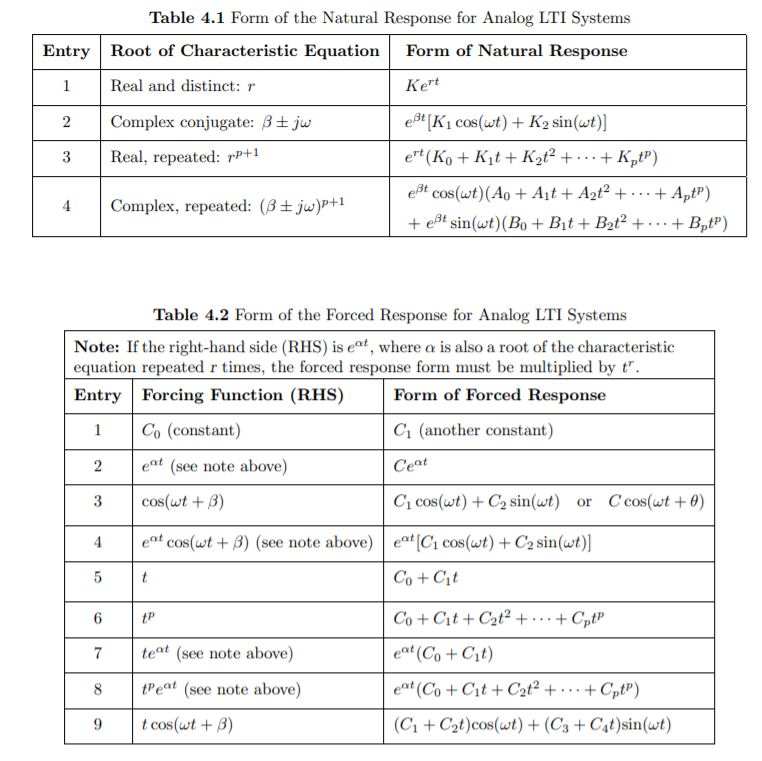
\includegraphics{Ne.JPG}
% \end{figure}
% \end{multicols}
\begin{figure}[H]
    \centering
    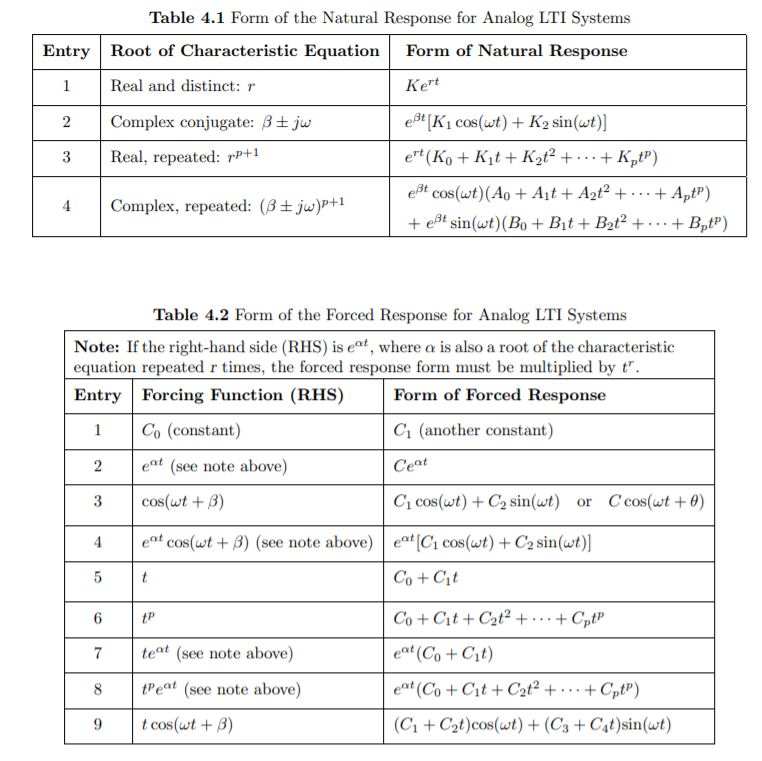
\includegraphics{Ne.JPG}
\end{figure}
\cleardoublepage

\section{Laplace Transform}
\begin{gather*}
    \mathscr{L}[f(t)]=F(s)=\int_0^\infty e^{-st}f(t)dt
\end{gather*}
\section{LPF: }
\begin{gather*}
    y(s)=X(s)*\frac{Z_c}{Z_R+Z_c}\\
    H(s)=\frac{\frac{1}{\tau}}{s+\frac{1}{\tau}}\\
    \frac{d}{dQ}\rightarrow y(s)[s+\frac{1}{\tau}]=\frac{1}{\tau}X(s)\\
    \mathscr{L}\rightarrow y(t)^{'}+\frac{1}{\tau}y(t)=\frac{x(t)}{\tau}\\
    h(t)=\frac{1}{\tau}e^{\frac{-t}{\tau}}u(t)\\
    y_{step}=\int_0^th(t)dt=-1\int_0^t\frac{1}{\tau}e^{\frac{-t}{\tau}}dt =-(e^{\frac{-t}{\tau}}-1)
\end{gather*}
\section{BIBO (bounded-input,bounded output):}
\begin{enumerate}
    \item \textbf{Proper: }The highest derivative of input never exceed the highest derivative of output $\frac{P(s)}{Q(s)}$ degree of P never exceed the degree of Q.
    \item Poles should be inside of left hand side.
    \item h(t) must absolutely integrable.
\end{enumerate}
\textbf{Example:}
\begin{align*}
    H(s) &=\frac{s+1}{s^2+4} \text{not stable because of s=$\pm j$}\\
    H(s) &=\frac{s^3+2}{s^2+3s+2} \text{unstable because of H(s) is not proper}\\
    H(s) &=\frac{s+2}{(s+1)(s-3)}\text{unstable because RHP s=3}
\end{align*}
\textbf{Marginally stable: } if order of higher derivative of input exceeds the higher derivative of output.
\begin{gather*}
	\frac{d^2x}{dt^2}+2\alpha \frac{dx}{dt}+\omega^2=f(t)\\
	s^2+2\alpha s+\omega_0=0\\
	\zeta =\frac{\alpha}{\omega}\\
	\zeta_{settle}= \frac{u}{\zeta\omega_n}\\
	\% overshoot=100 e^{\frac{-2\pi}{\sqrt{1-\zeta^2}}}\\
	s_1=-\alpha+\sqrt{\alpha^2-\omega_0 ^2}\\
	s_2=-\alpha-\sqrt{\alpha^2-\omega_0 ^2}\\
	x_c=K_1e^{s_1t}+K_2e^{s_2t}\rightarrow \zeta>1\text{ overdamped}\\
	x_c=K_1e^{s_1t}+K_2te^{s_1t}\rightarrow \zeta=1\text{ critically damped}\\
	x_c=K_1e^{-\alpha t}cos(\omega_n t)+K_2e^{-\alpha t}sin(\omega _n t)\rightarrow \zeta<1 \text{ underdapmped}\\
	\omega _n=\sqrt{\omega _0^2-\alpha^2}\\
	\alpha=\frac{1}{2RC}\\
	\omega _0=\frac{1}{\sqrt{LC}}
\end{gather*}
\section{Initial value and final value Theorem:}
The initial value theorem predicts the initial value x(0+) of the signal x(t) from its strictly proper transform X(s) as \\
$$x(0+)=\lim_{s\to\infty} [sX(s)]$$\\
The final value theorem predicts the value of the time signal x(t) as $t\rightarrow \infty$ from its transform X(s) and reads\\
$$x(\infty)=\lim_{s\to0}[sX(s)]$$

\section{Fourrier Transform:}
\begin{gather*}
%     \omega=2\pi f\\
%     a_0=\frac{1}{T}\int^T_0
% f(t)dt\\
% a_n=\frac{2}{T}\int_0^Tf(t)cos(\pi\omega t)dt\\
% b_n=\frac{2}{T}f(t)sin(\pi \omega t)dt\\
X(f)=\int^{\infty}_{-\infty}x(t)e^{-j2\pi ft}dt\\
inverse_{transform}=x(t)=\int^{\infty}_{-\infty}X(f)e^{j2\pi ft}dt\\
e^{i\theta}=cos(\theta)+isin(\theta)\\
e^{-i\theta}=cos(\theta)isin(\theta)\\
sin(\theta)=\frac{1}{2}[e^{i\theta}-e^{-i\theta}]\\
cos(\theta)=\frac{1}{2}[e^{i\theta}+e^{-i\theta}]
\end{gather*}

\end{document}
